\section{大气的压强}\label{sec:5-10}

地球周围被一层很厚的空气包围着,这个空气层一直延伸到几千千米的高空,包围地球的空气层又叫做大气层,
我们就生活在这个大气海洋的最底层。

跟其他物质一样,空气也有质量。用抽气机抽出瓶里的空气,然后用夹子夹紧橡皮管,把瓶放在天平上,
加砝码使天平平衡(图 \ref{fig:5-38})。松开夹子,让外面的空气进到瓶里,天平就失去平衡。必须增加砝码,
才能使天平恢复平衡。这增加的砝码就等于瓶中空气的质量。

\begin{figure}[htbp]
    \centering
    \begin{minipage}{9cm}
    \centering
    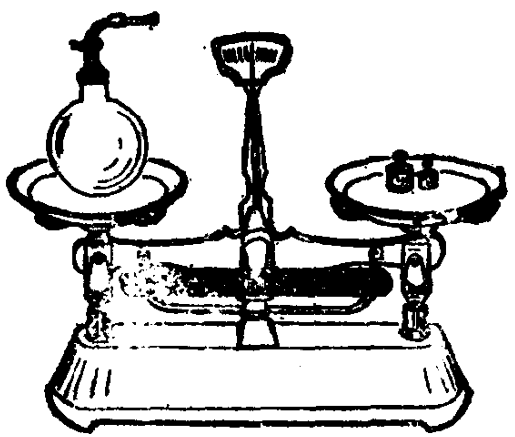
\includegraphics[width=6cm]{../pic/czwl1-ch5-38}
    \caption{}\label{fig:5-38}
    \end{minipage}
    \qquad
    \begin{minipage}{5cm}
    \centering
    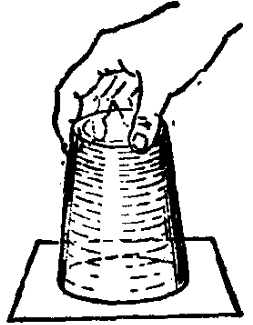
\includegraphics[width=4cm]{../pic/czwl1-ch5-39}
    \caption{}\label{fig:5-39}
    \end{minipage}
\end{figure}

在大气层里,空气的密度是随高度而变化的,越靠近地面越稠密,越到高空越稀薄。
因此,在地面附近空气的密度较大,随着高度的增加,密度越来越小。
在地面附近空气的密度大约是 $1.29 \qkmlfm$。

地球对空气也有吸引作用,因此,空气也受到重力。
所以象液体对浸在它里面的物体要产生压强一样,空气对浸在它里面的物体也要产生压强。
这个压强叫做\textbf{大气压强},简称\textbf{大气压}。

取一个盛满水的杯子,用纸片把杯口盖严,手按住纸片把杯子倒过来,放开手以后,纸片不会掉下来,杯子里的水也不会流出来(图 \ref{fig:5-39})。
这表明大气对纸片有向上的压力,这个力把纸片和水托住了。这个压力就是由大气压强产生的。

人们虽然很早就知道有空气,但在很长的时间内却不知道有大气压强。直到 17 世纪 40 年代才发现了大气压强。
但还是有许多人不相信。为了消除人们的怀疑,1654 年德国马德堡的市长、学者奥托·格里克表演了一个惊人的实验。
他把两个直径 30 多厘米的空心铜半球紧贴在一起,用抽气机抽出球内的空气,然后用两队马向相反的方向拉两个半球,
结果用了八对马还没有把它们拉开〈图 \ref{fig:5-40})。
\begin{figure}[htbp]
    \centering
    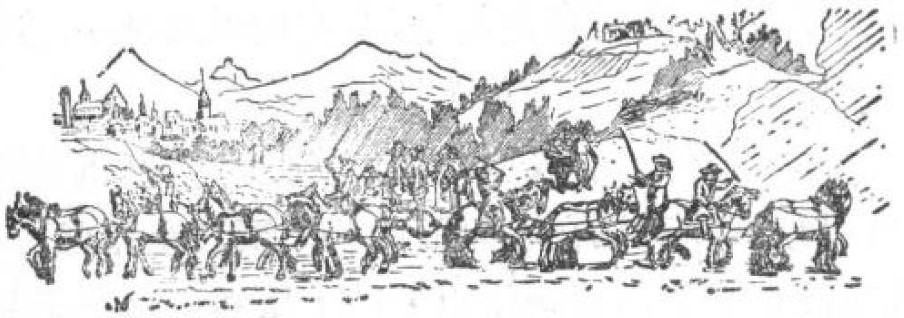
\includegraphics[width=0.7\textwidth]{../pic/czwl1-ch5-40}
    \caption{}\label{fig:5-40}
\end{figure}
球很不容易拉开,是因为球内的空气抽出以后,球里就没有空气的压强了,外面的大气压强就把两个半球紧紧地压在一起。
从这个实验可以看出,大气压强是很大的。
由于这个实验是在马德堡作的,后来就把这样的两半球叫做马德堡半球,把这个实验叫做马德堡半球实验。
马德堡半球实验有力地证明了大气压强的存在。
现在学校的实验室里也常常有马德堡半球,如果你们学校也有,同学们就可以自己来做这个实验,
抽出球内的空气后大家用力来拉,试试大气压强有多大。


